\documentclass[12pt]{article}

\usepackage{arxiv}

\usepackage[utf8]{inputenc} % allow utf-8 input
\usepackage[T1]{fontenc}    % use 8-bit T1 fonts
\usepackage{hyperref}       % hyperlinks
\usepackage{url}            % simple URL typesetting
\usepackage{booktabs}       % professional-quality tables
\usepackage{amsfonts}       % blackboard math symbols
\usepackage{nicefrac}       % compact symbols for 1/2, etc.
\usepackage{microtype}      % microtypography
\usepackage{lipsum}
\usepackage{graphicx}
\usepackage{listings}
\usepackage{cleveref}
\raggedbottom

\title{MosQEto: Machine Translation Quality Estimation Framework}


\author{
 Vilém Zouhar \\ \texttt{vilem.zouhar@mff.cuni.cz} \\
 \And
 Ondřej Měkota \\ \texttt{o@mkta.eu} \\
}

\begin{document}
\setlength{\headheight}{16pt}
\maketitle

\begin{abstract}
Word level quality estimation (QE) of machine translation is a task aiming to identify badly translated words and spaces between words. We propose a framework for experiment replication of QE systems MosQEto. We were also experimenting with several methods, trying to improve the quality estimation of systems implemented in OpenKiwi by smartly preprocessing and synthesizing training data. 
\end{abstract}

% keywords can be removed
\keywords{Quality Estimation \and Machine Translation \and WMT}

\section{Introduction}
Word level quality estimation is a task that receives the source of the translation and the translation itself and outputs which words in the output are translated correctly, usually in terms of probabilities. In WMT (since 2012) this is made into a classification task of every target token being either \texttt{OK} or \texttt{BAD}.

QE can be either supervised or unsupervised. The supervised version also gets the correct classification tags for each word and space between words during training. The unsupervised approaches rely mostly on getting self-reported confidence from machine translation models themselves. To our knowledge, this approach is much less reliable.

There are also document-level, paragraph-level, and sentence-level QE tasks. However, we did not consider those, because there are already ways of inferring higher-level estimations from word-level. We would also like to cast a shadow of doubt on this approach. It can often happen that every target word is part of a good translation, but the sentence as a whole is a bad translation. This can be supported by the fact that in BLEU, one can see examples of translations with very high bigram precision and very low or zero quadgram precision. From this perspective, sentence-level makes more sense. For sentence-level, HTER is used, which measures the amount of post-editing work needed to produce a good translation.

QE is becoming popular in translation companies for estimating post-editing costs.

\section{Word-level Quality Estimation}

In \cref{fig:example_qe_annotation} there is an illustration of word-level QE input, and output. Part of the QE task is to also predict missing words.

There are very few \texttt{BAD} tags, most word are translated correctly. Because of this imbalance $F_1$ is used for QE system evaluation. $F_1$ is computed separately for both \texttt{OK} tags (those that are classified as correctly translated) and \texttt{BAD} (those that are classified as incorrectly translated). These two computed numbers are then multiplied together yielding a $F_{MULTI} = F_{BAD} \cdot F_{OK}$ metric. Using $F_{MULTI}$ forbids cheating by e.g. only prediction \texttt{OK}, because $F_{OK}$ would be high, but $F_{BAD}$ zero. 

There are other possibilities of evaluation metrics, like mean square error, Spearman's, or Person's correlation, but they are used mostly for higher-level QE tasks.

The state of the art results for NMT QE models estimating for NMT MT models is $47.5\%$ for English-German \cite{fonseca2019findings}.

\begin{figure}[ht]
  \centering
  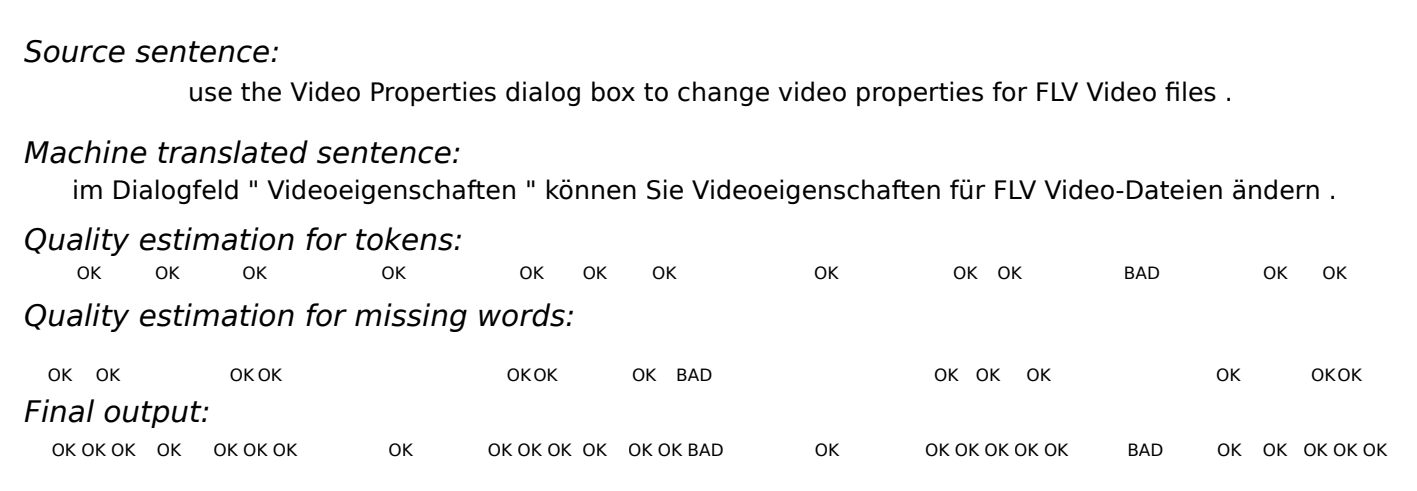
\includegraphics[width=\textwidth]{img/example_qe_annotation.png}
  \caption{Quality estimation example.}
  \label{fig:example_qe_annotation}
\end{figure}

\section{Quality Estimation Systems}

There are several architectures and tools to perform quality estimation: QuEst++ \cite{questplusplus}, DeepQuest \cite{deepquest} and OpenKiwi \cite{openkiwi}.

We have used OpenKiwi to perform our experiments because of the easy integration into our codebase. OpenKiwi is an open-source tool and contains four different architectures to do QE. We used only two: NuQE and QUETCH. This was so mainly because we did not aim to achieve the highest QE performance but only to compare our data preprocessing and synthesis tool with the baseline. PredEst and biRNN, the other models in OpenKiwi, take significantly more time to train.


\paragraph{QUETCH} First system that we used is a simple two layer neural network, the first layer has dimensionality 300 and the second 50.
It is fed word embeddings, of dimension 50 in our case, and it outputs probability distribution over \texttt{OK}/\texttt{BAD} tags.

\paragraph{NuQE} On top of four densely connected layer, NuQE contains also bi-directional GRU layer.
Because of the GRU layer, NuQE takes significantly more time to train compared to QUETCH.

\pagebreak

\section{MosQEto}
MosQEto is an open source\footnote{Contributions, and usage reports welcome at  \href{https://github.com/zouharvi/MosQEto}{github.com/zouharvi/MosQEto}} framework which allows researches to perform experiments defined by a simple YAML file. This YAML file represents a set of data and a processing pipeline. The pipeline can contain functions that process the data and perform training, testing, printing debugging messages.

The whole project is also integrated with fast\_align \cite{fastalign:2013} so that word alignment can be easily generated without any additional work from the experiment designer.

\begin{lstlisting}[caption={Example config file for data synthesis in MosQEto}, label={lst:experiment_def_example}, escapeinside={\%*}{*)}, stringstyle=\ttfamily, showstringspaces=false,captionpos=b]
dataset_load:
  - "opus/tech/en-de"
  - "wmt19/en-de"

dataset_save: 
  - "data_all/"
  
method:
  - Loader:rmdir:data_tmp
  - Loader:load:noalign
  - DataUtils:info
  - Generator:synthetize_random
  - DataUtils:head:7000
  - DataUtils:info
  
  - Loader:load
  - DataUtils:info
  
  - Generator:mix
  - Loader:save
  
generator:
  change_prob: 0.12
\end{lstlisting}

The example configuration file in \cref{lst:experiment_def_example} has a stack of two datasets: WMT19 QE annotated data and OPUS IT domain \cite{opus:2012}. They are loaded in order by calling \texttt{Loader:load} (each call loads one dataset into the buffer). QE data is synthesized from the OPUS dataset, cropped to 7000 units, and mixed with WMT19 QE data. 

\subsection{Commands}

Here we list the available commands in MosQEto experiment definitions.

\begin{itemize}
    \item \texttt{Loader:rmdir:D} removes the \texttt{D} directory. In MosQEto we used \texttt{data\_tmp} for intermediate results storage.
    
    \item \texttt{Loader:load} loads a new dataset from the top of the stack. Optionally \texttt{:noalign} can be specified to skip fast\_align invocation as it takes quite some time to finish. The corpora are loaded and downloaded dynamically. Thus, the user of MosQEto does not have to go through the process of manually downloading and unpacking datasets.
    
    \item \texttt{Loader:save} saves the current working data to a directory contained at the top of the save stack.
    
    \item \texttt{DataUtils:info} prints basic statistics about the data such as the distribution of \texttt{OK} and \texttt{BAD} tags. This command was crucial to us for data analysis.
    
    \item \texttt{DataUtils:flush\_train} removes the \texttt{train} part from the dataset.
    
    \item \texttt{DataUtils:split\_dev:P} moves P\% of the \texttt{train} units to \texttt{dev} part.
    
    \item \texttt{DataUtils:head:N} takes the first \texttt{N} units from the top of the dataset. 
    
    \item \texttt{Generator:synthetize\_random} acts according to the \texttt{generator} object which can contain \texttt{change\_prob}, \texttt{remove\_prob} and \texttt{append\_prob} for change, removal or insertion of words respectively. It takes every pair of (sentence, translation) and executes the given operation. For example in \cref{lst:experiment_def_example} it changes each target word with the probability 12\% and sets the corresponding tag to \texttt{BAD}. Other tags are set to \texttt{OK}.
    
    \item \texttt{Generator:expand\_post\_edited} simply takes all the post-edited sentences and sets their tags as \texttt{OK}.
    
    \item \texttt{Generator:synthetize\_gold} Marks every target token as \texttt{OK} or \texttt{BAD} based on whether it appears in the post-edited text. Optionally if the \texttt{generator} object has \texttt{case\_insensitive} set to \texttt{True} then the equivalency is compared without case sensitivity.
    
    \item \texttt{Generator:mix} shuffles the dataset. 
\end{itemize}

\section{Experiments}

We experiment with two datasets: the WMT19 Quality Estimation dataset (IT domain) and the OPUS from Ubuntu, PHP, KDE4, and Gnome \cite{opus:2012}. WMT19 contains 14 thousand parallel sentences and also post-edited sentences. Our part of OPUS on which we focused contains 300 thousand parallel sentences.

We experimented with dataset transformations and with transfer learning. All the experiments are documented\footnote{\href{https://github.com/zouharvi/MosQEto/blob/master/docs/experiments.md}{github.com/zouharvi/MosQEto/blob/master/docs/experiments.md}} in our GitHub repository together with the experiment definitions\footnote{\href{https://github.com/zouharvi/MosQEto/tree/master/config}{github.com/zouharvi/MosQEto/tree/master/config}} which can be used to reproduce our results.

\paragraph{Baseline} Our baseline is training QUETCH for $30$ epochs, the $F1_{MULTI}$ is $28.8\%$ and none of our experiments surpassed it.
We used Adam optimizer \cite{adam} with learning rate $10^{-4}$, $0.1$ dropout, and batch size $64$.

\paragraph{Small OPUS only with changes} We also trained a model on the OPUS dataset but preprocessing it such that for each word, a tag was switched to "BAD" with $12\%$ probability.
The F1 score was $16\%$.

\paragraph{WMT19 + WMT19 post-edited} The next experiment was training on WMT19 extended by the post-edited sentences, all marked "OK". 
This, however, did not improve the F1 score: $25.1\%$.

\paragraph{WMT19 + Small OPUS only with changes} Another experiment combined WMT19 data with those OPUS preprocessed data (with $12\%$ tag change to "BAD"). This setup matched the baseline performance, $28.8\%$.

\paragraph{WMT19 + PE synth} WMT19 was enriched by WMT19 data with different tags: a word is marked "OK" if and only if the word also appears in the post-edited version, "BAD" otherwise. This results in $25.9\%$ F1 score.

\paragraph{Transfer Learning} The transfer learning experiment failed badly. 
We suspect it is due to an error in the OpenKiwi framework.
We trained for 30 epochs on OPUS, and then for another 30 epochs on WMT19 and evaluated on WMT19.
The F1 was only $7\%$, which is $4$ times lower than the baseline.
This was after extensive hyperparameter search and even after using NuQE instead of QUETCH.
We tried to identify the error by trying to train on WMT19, save the model, and train again on WMT19, but there was still a drop in F1.

\section{Conclusion}

Even though we did not achieve any improvements over the baseline, we managed to implement (most of our dev time spent here) a robust system for experiment replication. An experiment of any kind (training, testing, data creation) can be easily defined using a single YAML file. MosQEto is oriented for data manipulation, but it can be used for anything if relevant \texttt{Worker} classes are implemented.

In our future work we would like to revise what went wrong with the transfer learning and come up with new ways of QE data synthesis. We mostly hoped for the post-edited data synthesis, but that failed.

% REFERENCES
\pagebreak
\bibliographystyle{apalike}
\bibliography{references}

\end{document}
